\thispagestyle{empty}

\section{Softwarelösungen}

\subparagraph{Linux-V Server}
Linux-VServer ist eine der ältesten Implementierungen von Linux-Container-basierten Systemen. Anstatt Namespaces zu verwenden, verwendet Linux-VServer selbst eingeführte Funktionen im Linux-Kernel um die Isolation zu gewähleisten, wie z.B. Prozessisolation, Netzwerkisolation und CPU-Isolation. Linux-VServer verwendet den tratidionellen Aufruf des Chroot-Systems, um das File-System innerhalb der Container einzusperren. Auf diese Weise schränkt es den Umfang des File-Systems für die Prozesse ein. Die Prozessisolierung erfolgt durch einen globalen PID-Raum, der alle Prozesse außerhalb des Bereichs eines Containers verbirgt und unerwünschte Verbindungen zwischen Prozessen verschiedener Container verhindert. Das wichtigste Merkmal dieses Ansatzes ist die Skalierbarkeit für eine große Anzahl von Containern. Der Nachteil ist jedoch die Unfähigkeit des Systems die üblichen Virtualisierungstechniken wie Live-Migration, Checkpoint und Wiederherstellung zu implementieren, da es nicht möglich ist, Prozesse mit derselben PID neu zu initiieren. Linux-VServer virtualisiert keine Netzwerk-Subsysteme. Vielmehr werden alle Netzwerk-Subsysteme (wie Routingtabellen und IP-Tabellen) von allen Containern gemeinsam genutzt. Dieser Ansatz setzt einen Identifier-Tag um zu vermeiden, dass ein Container Netzwerkverkehr zu anderen Containern empfangen kann. Entsprechende Filter sind im Netzwerk stack hinterlegt, um sicherzustellen, dass nur der richtige Container die Daten empfangen kann. Die Container sind nicht in der Lage ihre eigenen Routingtabellen-und IP-Tabellen zu ändern, was vom Host-Administrator durchgeführt werden muss. Um die CPU-Isolation zu gewährleisten, verwendet Linux-VServer den Standard-Linux-Scheduler, der durch das Token Bucket Filter (TBF) Schema überlagert wird. Jedem Container ist ein Token Bucket zugeordnet, der dazu dient, Token mit einer bestimmten Geschwindigkeit zu sammeln. Auf diese Weise ist jeder Prozess, bei der Erstellung eines Token mit einem Container verbunden. Diese Token werden bei der Ausführung auf der CPU im Container-Bucket bis zu einer bestimmten Mindest- oder Maximalanzahl gesammelt. Dieses Token-Bucket-Schema kann verwendet werden, um eine faire Aufteilung der CPU zu gewährleisten. Ressourcenbegrenzungen wie Speicherverbrauch und Anzahl der Prozesse werden mit Systemaufrufen (rlimit-Tool) des Linux-Kernels durchgeführt. Die neuesten Versionen von Linux-VServer bieten jedoch Unterstützung für Cgroups, mit denen auch die CPU-Auslastung und der Speicherverbrauch von Containern eingeschränkt werden können. Die Linux-VServer-Container werden vom util-vserver\cite{Optionen2018Userspace-WerkzeugeLinux-VServer} package verwaltet \cite{Overview2018PaperLinux-VServer} \cite{Xavier2015AClouds}.

\subparagraph{Open VZ}
penVZ bietet eine ähnliche Funktionalität wie Linux-VServer. Es basiert jedoch auf Kernel-Namespaces, wodurch es sicherstellt, das jeder Container seine eigene isolierte Teilmenge einer Ressource erhällt. Das System verwendet PID-Namespaces, um die Prozessisolierung zwischen Containern zu gewährleisten. Darüber hinaus ermöglichen PID-Namespaces übliche Virtualisierungstechniken wie Live-Migration, Checkpoint und Widerherstellungs Methoden. In OpenVZ hat dank IPC-Namespaces jeder Container sein eigenes Speicher, Semaphoren und Nachrichten Segment. Außerdem werden Network-Namespaces genutzt. OpenVZ verwendet vier Ressourcenmanagement Komponenten, "User Beancounter" (UBS), faires CPU-Scheduling, "Disk Quatas" und I/O-scheduling. UBS bietet die Möglichkeit der Limitierung der Ressourcen, die auf jedem Container kontrolliert werden. Der OpenVZ CPU scheduler funktioniert auf zwei arten um eine faire verteilung zu generieren. Zum einen wird entschieden welcher Container als nächstes auf dem Processor ausgeführt werden darf, zum anderen wird anhand einer Prioritätenliste die Reihenfolge der Prozesse des Containers erstellt. Es gibt eine weiteres Konzept ist die "VCPU Affinity", was die maximale Anzahl an CPUs definiert, die ein Container verwenden darf. "Disk Quota" ist eine Funktion, mit der eine Begrenzung des Speicherplatzes auf einem Speichermedium für einzelne Benutzer oder eine Gruppe von Benutzern festgelegt werden kann. Schließlich wird ein ähnlicher Ansatz des CPU-scheduling für I/O-scheduling verwendet. Das Verfahren ist wieder in zwei Teile aufgeteilt, der erste Teil funktioniert genau wie beim CPU-scheduling, der zweite teil wird anhand des "Completely Fair Queuing" (CFQ) Algorithmus festgelegt. Jeder Container besitzt eine I/O-Priorität, und der I/O-Scheduler verteilt die verwendbare Bandbreite anhand der Priorisierung. Auf diese weise kann nicht ein Einzelner Container die Kompletten Kanal beanspruchen. OpenVZ Container werden durch "vzctl"\cite{ParallelsIPHoldingsGMbH2018Vzctl} verwaltet\cite{IndexOpenvz.org}\cite{Xavier2015AClouds}.

\subparagraph{Linux Container}
Ähnlich wie Open VZ verwendet LXC Kernel-Namespaces, um die Ressourcenisolierung zwischen allen Containern zu gewährleisten. Während des Container Starts, werden stanardmäßig PIDs, IPCs und Mount Points virtualisiert und über den PID-Namespace, den IPC-Namespace bzw. den Mount-Namespace isoliert. Um mit der Außenwelt zu kommunizieren und die Netzwerkisolierung zu ermöglichen, werden verwendet LXC die Nezwerk-Namespaces. Im gegensatz zu Linux-VServer und OpenVZ ist die Ressourcenverwaltung nur über Cgroups erlaubt. Die Prozesskontrolle wird ebenfalls über Cgroups durchgeführt. I/O Operationen sind wie in OpenVZ ebenfalls durch den CFQ-scheduler gesteuert \cite{IndexLinuxcontainers.Org} \cite{Xavier2015AClouds}.

\vspace{1em}
\begin{minipage}{\linewidth}
	\centering
	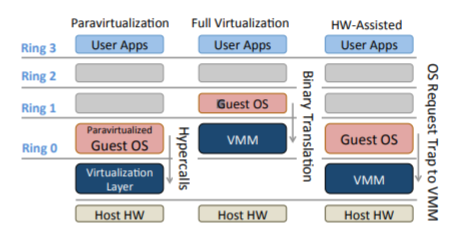
\includegraphics[width=1\linewidth]{pics/Virtualisierungen_Hypervisor.PNG}
	\captionof{figure}[Virtualisierungen Hypervisor]{Virtualisierungen Hypervisor \cite{Fayyad-Kazan2013BenchmarkingHypervisors}}
	\label{fig:Virtualisierungen_Hypervisor}
\end{minipage}

\subparagraph {Xen}
Xen ist eine Virtualisierungslösung, die ursprünglich an der University of Cambridge entwickelt wurde. Xen ist die einzige Bare-Metal-Lösung, die als Open Source als Grundlage für eine Reihe verschiedener Kommerzieller und Open-Source-Anwendungen dient. Xen besteht aus mehreren Komponenten, die zusammenwirken, um eine Virtualisierungsumgebung bereitzustellen. Die Hauptbestandteile sind Xen-Hypervisor, Domain0 Gast (Dom0) und DomainU Gast (DomU), die entweder Para-Virtualisiert, Vollständig-Virtualisert oder Hardwareunterstützt-Virtualisiert sein können. Der Xen-Hypervisor ist eine Softwareschicht, die direkt auf der Hardware unter allen Betriebssystemen läuft. Er ist für das CPU-Scheduling und die Speicherpartitionierung der verschiedenen VMs die auf der Hardwarevorrichtung laufen zuständig. Wenn Xen startet, übernimmt der Xen-Hypervisor die Kontrolle über das System und lädt das erste Gastbetriebssystem auf Dom0. Dom0 ist ein modifizierter Linux-Kernel, der eine einzigartige Virtuelle Maschine darstellt und auf dem Xen-Hypervisor mit speziellen Zugriffsrechten auf physische I/O-Ressourcen, sowie die Interaktion mit anderen virtuellen Maschinen läuft. Die auf der DomU ausgeführten modifizierten Betriebssysteme, besitzen keinen direkten Zugriff auf physische Daten.Seit Xen Version 3.0 ist CREDIT der Standat Xen-Scheduler um die CPU fair auf den Virtuellen Maschinen aufzuteilen. Im Credit-Scheduler wird jeder VM eine Gewichtung zugewiesen, anhand dieser werden die CPU-Ressourcen auf die Systeme verteilt\cite{Fayyad-Kazan2013BenchmarkingHypervisors}. 

\subparagraph {VMware ESXi \cite{Fayyad-Kazan2013BenchmarkingHypervisors}}
VMware vSphere ist eine Software-Lösung mit folgenden Funktionen


\subparagraph {VMware Workstation}
\subparagraph{Virtual Box}


\subparagraph{KVM}
Kernel Virtual Machine (KVM) ist eine Funktion von Linux, die es ermöglicht als typ-1-Hypervisor zu fungieren und ein unmodifiziertes gast Betriebssystem in einem Linux Prozess zu erstellen. KVM verwendet Hardware-Virtualisation in aktuellen Prozessoren um die Komplexität und den Overhead zu reduzieren. Bei Intel VT-x oder AMD-v erübrigt sich die Notwendigkeit einer komplexen Ring-Rechteverwaltung, welches von früheren Hypervisoren wie Xen und VMware verwendet wurde. KVM verwendet sowohl über "QEMU\cite{QEMUEmulator}" emolierte, als auch via "virtio\cite{View2018VirtioVirtio}" paraviertualisierte I/O-Geräte. Die Kombination aus Hardwarebeschleunigung und Paravirtuellem I/O ist ist entwickelt worden, um den Virtualisierungs-Overhead auf shr niedrige Werte zu reduzieren. KVM unterstützt die Live-Migration und ermöglicht dadurch die Wartung von physischen Servern oder sogar ganzen Rechenzentren, ohne dass einGastbetriebssystem unterbrochen wird. Da eine VM eine statische Anzahl von virtuellen CPUs (vCPUs) hat und eine feste Menge an Arbeitsspeicher, ist der Ressourcenverbrauch natülich begrenzt. Eine vCPU stellt einen echten CPU-Wert der Zyklen dar und jede Memory-Page des virtuellen Arbeitsspeichers stellt genau eine Memory-Page des realen Rechners dar. KVM kann die Größe von VMs während des Betriebs durch "Hotplugging" und "Ballooning" durch die dafür benötigte Betriebssystemunterstützung verändern. Da jede VM ein Prozess ist, gelten alle normalen Linux-Ressourcenverwaltungsfunktionen in den Virtuellen Maschinen. Das vereinfacht zwar die Implementierung und Verwaltung des Hypervisors, erschwert aber die Ressourcenverwaltung innerhalb des Gastbetriebssystems. Betriebssysteme gehen im Allgemeinen davon aus, dass CPUs immer laufen und der Speicher eine relativ feste Zugriffszeit hat, aber unter KVM können vCPUs ohne Benachrightigung ausgeplant werden, was zu Performance-Anomalien führt, die schwer zu debuggen sind. Viele Cloud-Anbieter beseitigen diese Probleme, indem sie keine übermäßigen Ressourcen binden, jede vCPU an eine physische CPU koppeln und den gesamten virtuellen Arbeitsspeicher auf den Realen zuschneiden. Dadurch entfällt im Wensentlichen die Planung im Hypervisor. VMs bieten ein gewisses Maß an Isolierung und Sicherheit durch ihre schmale Schnittstelle. Der einzig Weg über die eine VM mit der Außenwelt kommunizieren kann ist über eine begrenzte Anzahl von Hypercalls oder emulierten Geräten, die beide vom Hypervisor gesteuert werden. Doch auch das ist keine Perfekte Lösung, es wurden Hypervisor-Privilegien-Eskalationsschwachstellen entdeckt, die es einem Gastbetriebssystem ermöglichen konnten aus seiner VM "Sandbox" auszubrechen\cite{Felter2014IBMContainers}.

\subparagraph{Hyper-V}
Microsoft Hyper-V ist ein in Windows integrierter Hypervisor, der die Möglichkeit für Para-Virtualisierung und Hardwareunterstütze-Virtualisierung bereitstellt. Hyper-V gibt es zudem als Eigenständie Version namens Hyper-V Server und als Installierbares Produkt "Windows Server" Es gibt keine Unterschiede in der Funktionsweise zwischen den Microsoft Hyper-V, der Hypervisor ist der selbe unabhängig von der installierten Variante. MS Hyper-V implementiert die Isolierung von virtuellen Maschinen in Form von Partitionen (Betriebssystem und Anwendungen). Hyper-V unterstütz Para-Virtualisierung und Hardware-Virtualisierung. Genau wie bei KVM kann der Performance Overhead reduziert werden. Die Architektur des Hyper-V funktioniert anhand von micro-kernelized Hypervisoen. Bei dieser Architektur wird ein Parant/Child system verwendet, wobei die Parent Partition das Management von Hardware Geräten organisiert. Das original erstellte Windows Betriebssystem stellt die Parent Partition dar, alle weiteren neu erstellten Virtuellen Maschinen bilden die sogenannten Child-Partitionen. Jeder zugrif auf virtuelle Geräte wird vom VMBus dirigiert. VMBus ist ein logischer channel welcher die inter-Partitions-Kommunikation verhinder und nur mit berechtigten Partitionen interagiert. Auch der durch Hyper-V zur Verfügung gestellt Hypervisor konnte von einem User der aus der "Sandbox" des Gastbetriebssystem entkommen konnte und Privilegierten Zugriff auf Ressourcen hatte\cite{Fayyad-Kazan2013BenchmarkingHypervisors}. 